\section{Visitor}

O padrão Visitor define uma estrutura que permite realizar 
operações em uma estrutura de objetos sem precisar alterá-los 
e sem precisar que os objetos dessa estrutura conheçam as 
operações que estão sendo realizadas. 

Uma estrutura alvo de um Visitor pode possuir objetos de 
classes diferentes. Por isso, o padrão deve implementar 
uma operação \textit{visit} para cada uma dessas classes, 
através de uma sobrecarga de métodos. Para que essa 
abordagem funcione, as classes da estrutura devem implementar 
uma operação \textit{accept} que recebe como parâmetro um 
Visitor genérico e chama sua operação \textit{visit}, 
passando uma referência para a instância atual (this) 
como parâmetro. Dessa forma, a função chamada é a 
que recebe a classe em questão como parâmetro.

Esse padrão permite estender objetos para novas operações 
sem comprometer sua implementação ou poluir as classes com 
diversas operações que não são de sua responsabilidade. 
Sua estrutura pode ser vista na imagem \ref{visitor_struct}.

\begin{figure}[htb]
	\caption{\label{visitor_struct}Estrutura do Visitor}
	\begin{center}
	    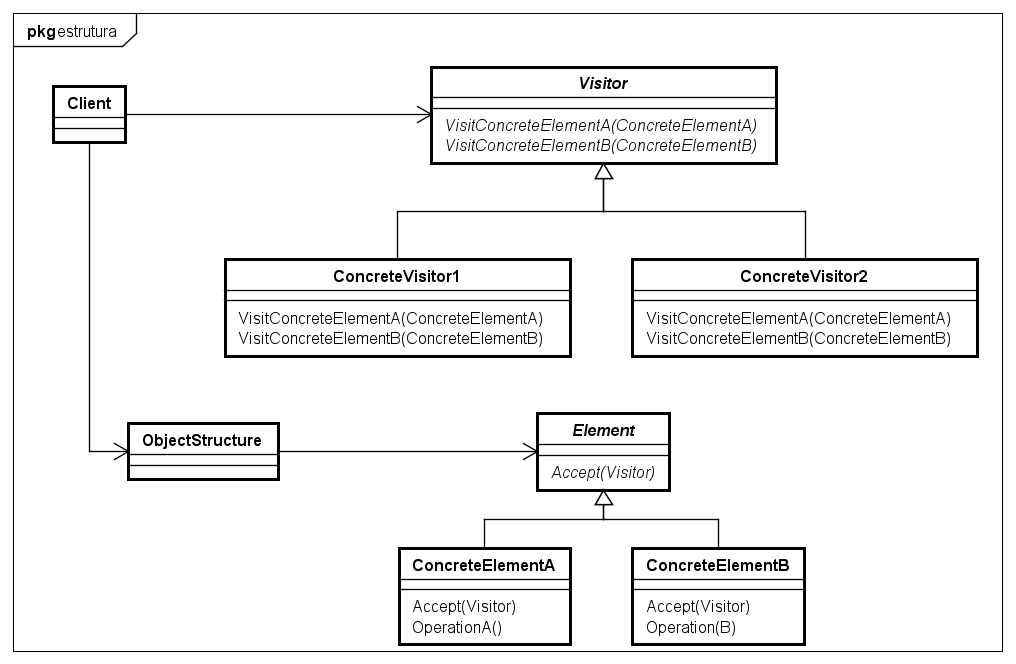
\includegraphics[scale=0.5]{5_padroes-contexto-funcional/5.3_comportamentais/5.3.11_visitor/visitor_estrutura.png}
	\end{center}
\end{figure}

\subsection*{Exemplo Orientado a Objetos}

Um compilador precisa fazer a análise de árvore abstrata sintática de 
um programa. Essa análise inclui diversas operações diferentes, como 
checagem de tipos e geração de código. Para que os nós da árvore 
não precisem implementar essas operações, elas implementam uma operação 
genérica que recebe como parâmetro qualquer Visitor. Dessa forma, para 
cada operação desejada, basta implementar uma nova classe Visitor 
que percorrerá os elementos da árvore abstrata sintática. O diagrama 
de classes para o exemplo pode ser visto na imagem \ref{visitor_exemplo1}, 
enquanto a implementação pode ser vista no código \ref{oovisitor}.

\begin{figure}[htb]
	\caption{\label{visitor_exemplo1}Exemplo de Visitor}
	\begin{center}
	    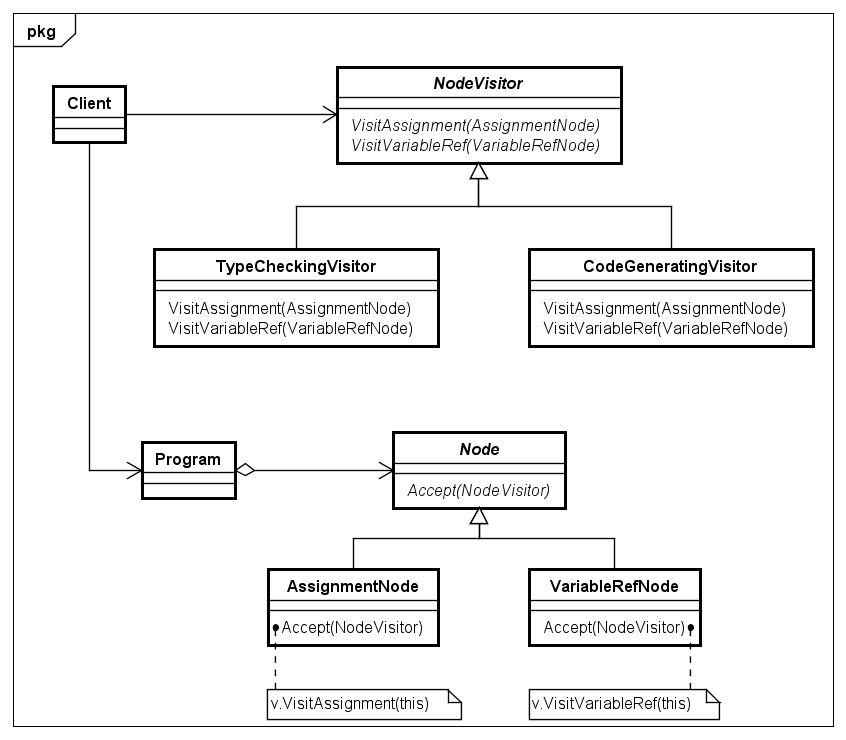
\includegraphics[scale=0.5]{5_padroes-contexto-funcional/5.3_comportamentais/5.3.11_visitor/visitor_exemplo.png}
	\end{center}
\end{figure}

\begin{lstlisting}[caption={Visitor Orientação a Objetos},label=oovisitor]

trait NodeVisitor {
  def VisitAssignment(node : AssignmentNode)
  def VisitVariableRef(node : VariableRefNode)
}

trait Node {
  def Accept(visitor : NodeVisitor)
}

class AssignmentNode extends Node {
  def Accept(visitor: NodeVisitor): Unit = visitor.VisitAssignment(this)
}

class VariableRefNode extends Node {
  def Accept(visitor : NodeVisitor) : Unit = visitor.VisitVariableRef(this)
}

class TypeCheckingVisitor extends NodeVisitor {

  def VisitAssignment(node: AssignmentNode): Unit = {
    //Operações de checagem de tipo para atribuição
  }

  def VisitVariableRef(node: VariableRefNode): Unit = {
    //Operações de checagem de tipo para variáveis
  }
}

class CodeGeneratingVisitor extends NodeVisitor {

  def VisitAssignment(node: AssignmentNode): Unit = {
    //Operações de geração de código para atribuição
  }

  def VisitVariableRef(node: VariableRefNode): Unit = {
    //Operações de geração de código para variáveis
  }
}

\end{lstlisting}

\subsection*{Contexto Funcional}

Uma das maiores vantagens do padrão Visitor 
é o uso de multimétodos, onde um método é 
executado de forma dinâmica, baseado no tipo 
de um objeto em tempo de execução. Essa 
funcionalidade é possível através do polimorfismo 
nas linguagens orientadas a objetos.\cite{gamma:1995}

Uma funcionalidade semelhante que algumas 
linguagens funcionais implementam é o 
\textit{pattern matching}\cite{realworldhaskell,
functionalscala}. 
Ela consiste em avaliar um valor a partir de 
um padrão predefinido, ou seja, a operação 
que será realizada dependerá do valor avaliado
\cite{functionalscala}. 
No caso do padrão Visitor, todos os métodos 
sobrecarregados que executam a operação 
em cada tipo de elemento da coleção são 
substituídos por um único método que 
reconhece o tipo de valor da estrutura. 
Essa abordagem possui suas desvantagens, 
dependendo de como a linguagem implementa 
o \textit{pattern matching}. No caso de Scala, 
pode ser necessário incluir nos valores da 
estrutura um valor enumerável que identifica o 
tipo do elemento. 

O código \ref{fpvisitor} demonstra como o 
exemplo orientado a objetos pode ser implementado. 
O tipo Node, definido na linha 2, armazena um valor 
enumerável com os tipos de nó suportados 
pela aplicação, além dos outros valores 
armazenados por um nó - representados pelo tipo 
NodeValue. A função DefineNodeVisitor, definida 
na linha 4, aproveita o uso de funções de alta ordem 
para gerar tipos diferentes de Visitor. Ela 
recebe como parâmetro duas funções, uma que 
realiza uma operação para o tipo de nó Assignment e 
outra que realiza uma operação para o tipo de 
nó VariableRef. Ela retorna uma nova função - o 
Visitor - que recebe como parâmetro uma coleção 
de nós e retorna a mesma coleção após aplicadas 
todas as operações. Nas linhas 9 e 11 é onde 
ocorre o \textit{pattern matching}. Uma operação 
de desconstrução é aplicada na tupla que representa 
um nó. Caso o nó seja do tipo Assignment, o 
primeiro caso é executado. Caso seja do tipo 
VariableRef, o segundo caso é executado.

\begin{lstlisting}[caption={Visitor Funcional},label=fpvisitor]
    
type Node = (NodeType.Value, NodeValue)

def DefineNodeVisitor(AssignmentNodeVisitor : NodeValue => Node,
                      VariableRefNodeVisitor : NodeValue => Node) :
List[Node] => List[Node] = {
  (nodes : List[Node]) => {
    nodes.map {
      case (NodeType.AssignmentNode, value) => 
        AssignmentNodeVisitor(value)
      case (NodeType.VariableRefNode, value) => 
        VariableRefNodeVisitor(value)
    }
  }
}
    
\end{lstlisting}